\documentclass[12pt,dvipdfmx]{beamer}

\usepackage{graphicx}
\DeclareGraphicsExtensions{.pdf}
\DeclareGraphicsExtensions{.eps}
\graphicspath{{out/tex/svg/}{out/pdf/svg/}}
\usepackage{listings}
\usepackage{fancybox}
\usepackage{hyperref}
\usepackage{color}

\newcommand{\plusequal}{\mbox{\tt\ += }}
\newcommand{\minusequal}{\mbox{\tt\ -= }}
\newcommand{\divequal}{\mbox{\tt\ /= }}
\newcommand{\plusplus}{\mbox{\tt\ ++ }}



%% OpenMP section numbers
\newcommand{\sectionompparallel}{2.5}
\newcommand{\sectionompdeterminenumthreads}{2.5.1}
\newcommand{\sectionompfor}{2.7.1}
\newcommand{\sectionompdataenv}{2.14}
\newcommand{\sectionompgetnumthreads}{3.2.2}
\newcommand{\sectionompgetmaxthreads}{3.2.3}
\newcommand{\sectionompgetthreadnum}{3.2.4}


%%%%%%%%%%%%%%%%%%%%%%%%%%%
%%% themes
%%%%%%%%%%%%%%%%%%%%%%%%%%%
%\usetheme{Szeged} 
\usetheme{Madrid}

%% no navigation bar
% default boxes Bergen Boadilla Madrid Pittsburgh Rochester
%% tree-like navigation bar
% Antibes JuanLesPins Montpellier
%% toc sidebar
% Berkeley PaloAlto Goettingen Marburg Hannover Berlin Ilmenau Dresden Darmstadt Frankfurt Singapore Szeged
%% Section and Subsection Tables
% Copenhagen Luebeck Malmoe Warsaw

%%%%%%%%%%%%%%%%%%%%%%%%%%%
%%% innerthemes
%%%%%%%%%%%%%%%%%%%%%%%%%%%
% \useinnertheme{circles}	% default circles rectangles rounded inmargin

%%%%%%%%%%%%%%%%%%%%%%%%%%%
%%% outerthemes
%%%%%%%%%%%%%%%%%%%%%%%%%%%
% outertheme
% \useoutertheme{default}	% default infolines miniframes smoothbars sidebar sprit shadow tree smoothtree


%%%%%%%%%%%%%%%%%%%%%%%%%%%
%%% colorthemes
%%%%%%%%%%%%%%%%%%%%%%%%%%%
\usecolortheme{seahorse}
%% special purpose
% default structure sidebartab 
%% complete 
% albatross beetle crane dove fly seagull 
%% inner
% lily orchid rose
%% outer
% whale seahorse dolphin

%%%%%%%%%%%%%%%%%%%%%%%%%%%
%%% fontthemes
%%%%%%%%%%%%%%%%%%%%%%%%%%%
\usefonttheme{serif}  
% default professionalfonts serif structurebold structureitalicserif structuresmallcapsserif

%%%%%%%%%%%%%%%%%%%%%%%%%%%
%%% generally useful beamer settings
%%%%%%%%%%%%%%%%%%%%%%%%%%%
% 
\AtBeginDvi{\special{pdf:tounicode EUC-UCS2}}
% do not show navigation
\setbeamertemplate{navigation symbols}{}
% show page numbers
\setbeamertemplate{footline}[frame number]


%%%%%%%%%%%%%%%%%%%%%%%%%%%
%%% define some colors for convenience
%%%%%%%%%%%%%%%%%%%%%%%%%%%

%\newcommand{\mido}[1]{{\color{green}#1}}
\newcommand{\mido}[1]{{\color{green}#1}}
\newcommand{\mura}[1]{{\color{purple}#1}}
\newcommand{\ore}[1]{{\color{orange}#1}}
\newcommand{\ao}[1]{{\color{blue}#1}}
\newcommand{\aka}[1]{{\color{red}#1}}

\setbeamercolor{ex}{bg=cyan!20!white}

%%%%%%%%%%%%%%%%%%%%%%%%%%%
%%% how to typset code
%%%%%%%%%%%%%%%%%%%%%%%%%%%

\lstset{language = C,
numbers = left,
numberstyle = {\tiny \emph},
numbersep = 10pt,
breaklines = true,
breakindent = 40pt,
frame = tlRB,
frameround = ffft,
framesep = 3pt,
rulesep = 1pt,
rulecolor = {\color{blue}},
rulesepcolor = {\color{blue}},
flexiblecolumns = true,
keepspaces = true,
basicstyle = \ttfamily\scriptsize,
identifierstyle = ,
commentstyle = \it\scriptsize,
stringstyle = ,
showstringspaces = false,
tabsize = 4,
escapechar=\@,
}

\title{Understanding Task Scheduling Algorithms}
\institute{}
\author{Kenjiro Taura}
\date{}

\AtBeginSection[] % Do nothing for \section*
{
\begin{frame}
\frametitle{Contents}
\tableofcontents[currentsection,currentsubsection]
\end{frame}
}
\AtBeginSubsection[] % Do nothing for \section*
{
\begin{frame}
\frametitle{Contents}
\tableofcontents[currentsection,currentsubsection]
\end{frame}
}

\begin{document}
\maketitle

%%%%%%%%%%%%%%%%%%%%%%%%%%%%%%%%%% 
\begin{frame}
\frametitle{Contents}
\tableofcontents
\end{frame}

%=================================

%=================================

%=================================
\section{Introduction}
%=================================

%%%%%%%%%%%%%%%%% 
\begin{frame}[fragile]
\frametitle{Introduction}
\begin{itemize}
\item in this part, we study 
  \begin{itemize}
  \item how tasks in task parallel programs are scheduled
  \item what can we expect about its performance
  \end{itemize}
\begin{columns}
\begin{column}{0.5\textwidth}
\begin{lstlisting}
void @\ao{\tt ms}@(elem * a, elem * a_end, 
        elem * t, int dest) {
  long n = a_end - a;
  if (n == 1) {
    ...
  } else {
    ...
    @\ao{\tt create\_task(}@ms(a, c, t, 1 - dest)@\ao{\tt )}@;
    ms(c, a_end, t + nh, 1 - dest);
    @\ao{\tt wait\_tasks}@;
  }
}
\end{lstlisting}
\end{column}
\begin{column}{0.5\textwidth}
\begin{center}
%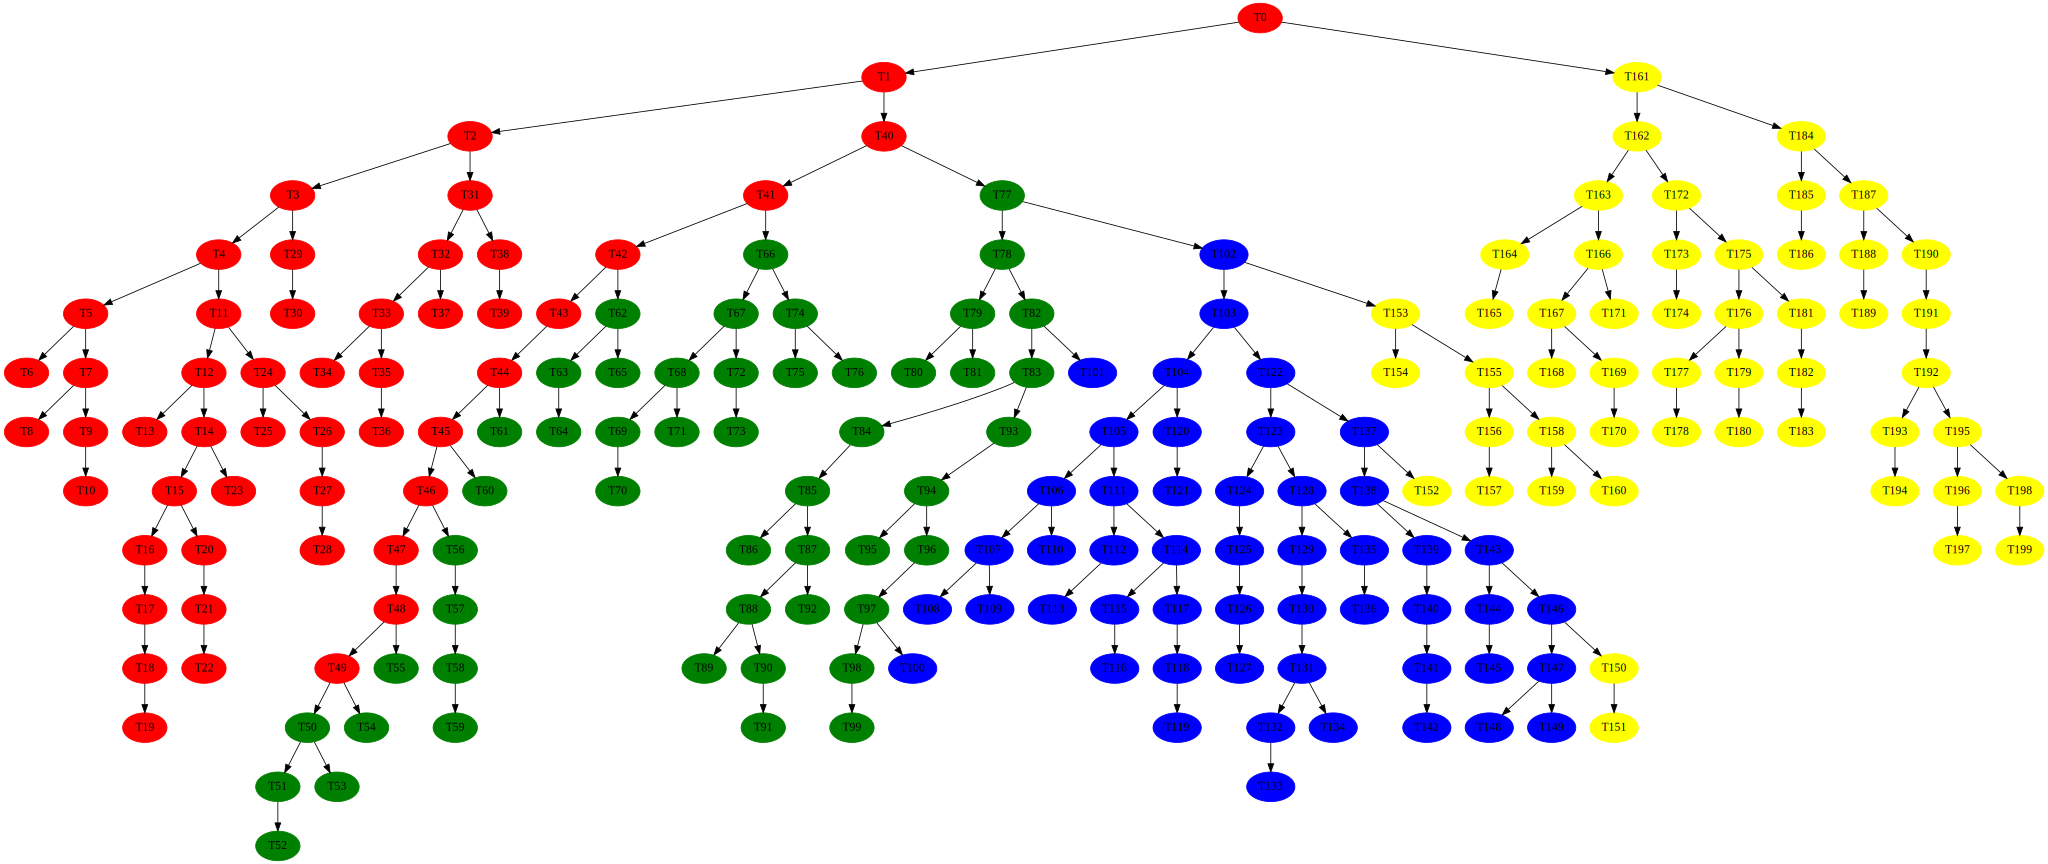
\includegraphics[width=0.8\textwidth]{out/pdf/svg/randtree.pdf}
\end{center}
\end{column}
\end{columns}
\end{itemize}
\end{frame}


%%%%%%%%%%%%%%%%% 
\begin{frame}
\frametitle{Goals}
\begin{itemize}
\item<1-> understand a state-of-the-art scheduling algorithm 
  \ao{\em (work stealing scheduler)}

\item<2-> \ao{execution time (without modeling communication):} 
  \begin{itemize}
  \item how much time does a scheduler take to finish a computation?
  \item in particular, \ao{\em how close is it to greedy schedulers?}
  \end{itemize}

\item<3-> \ao{data access (communication) cost:}
  \begin{itemize}
  \item when a computation is
    executed in parallel by a scheduler, 
    how much data are transferred (caches $\leftrightarrow$ memory,
    caches $\leftrightarrow$ cache)?
  \item in particular, how much are they 
    worse (or better) than those of the serial execution?
  \end{itemize}
\end{itemize}
\end{frame}

%=================================
\section{Work stealing scheduler}
%=================================

%%%%%%%%%%%%%%%%% 
\begin{frame}[fragile]
\frametitle{Model of computation}

\begin{itemize}
\item assume a program performs the following operations
  \begin{itemize}
  \item \ao{\tt create\_task($S$)}: create a task that performs $S$
  \item \ao{\tt wait\_tasks}: waits for completion of tasks 
    it has created (but has not waited for)
  \end{itemize}
\item e.g.,
\begin{lstlisting}
int fib(n) {
  if (n < 2) return 1;
  else {
    int x, y;
    create_task({ x = fib(n - 1); }); // share x
    y = fib(n - 2);
    wait_tasks;
    return x + y;
  }
}    
\end{lstlisting}
\end{itemize}
\end{frame}



%%%%%%%%%%%%%%%%% 
\begin{frame}[fragile]
\frametitle{Model of computation}

\begin{itemize}
\item model an execution as a DAG (directed acyclic graph)
  \begin{itemize}
  \item node: a sequence of instructions
  \item edge: dependency
  \end{itemize}

\item assume \aka{\em no other dependencies
    besides induced by {\tt create\_task($S$)} and
    {\tt wait\_tasks}}

\item e.g., (note $C_1$ and $C_2$ may be subgraphs, not single nodes)

\begin{columns}
\begin{column}{0.6\textwidth}
\begin{itemize}
\item []
\begin{lstlisting}
@$P_1$@
create_task(@$C_1$@);
@$P_2$@
create_task(@$C_2$@);
@$P_3$@
wait_tasks;
@$P_4$@
\end{lstlisting}
\end{itemize}
\end{column}
\begin{column}{0.4\textwidth}
\begin{center}
\def\svgwidth{0.4\textwidth}
{\scriptsize \input{out/tex/svg/dag_example.pdf_tex}}
\end{center}
\end{column}
\end{columns}
\end{itemize}
\end{frame}


%%%%%%%%%%%%%%%%% 
\begin{frame}
\frametitle{Terminologies and remarks}
\begin{columns}
\begin{column}{0.7\textwidth}
\begin{itemize}
\item a single node in the DAG represents 
  a sequence of instructions performing
  no task-related operations

\item note that a \ao{\em task} $\neq$ a single
  node, but $=$ \aka{\em a sequence of} nodes

\item we say \ao{\em a node is ready} when all its
  predecessors have finished; we say 
  \ao{\em a task is ready} to mean a node of it becomes ready
\end{itemize}
\end{column}
\begin{column}{0.3\textwidth}
\begin{center}
\def\svgwidth{0.8\textwidth}
{\footnotesize \input{out/tex/svg/dag_example_2.pdf_tex}}
\end{center}
\end{column}
\end{columns}
\end{frame}

%=================================
%\subsection{Work stealing scheduler}
%=================================

%%%%%%%%%%%%%%%%% 
\begin{frame}
\frametitle{Work stealing scheduler}
\begin{itemize}
\item a state of the art scheduler of task parallel systems
\item the main ideas invented in 1990:
  \begin{itemize}
  \item []
    Mohr, Kranz, and Halstead. 
    {\em Lazy task creation: a technique for increasing the granularity of parallel programs.}
    ACM conference on LISP and functional programming.
  \end{itemize}
\item originally termed ``Lazy Task Creation,'' 
  but essentially the same strategy is nowadays called ``work stealing''
\end{itemize}
\end{frame}


%%%%%%%%%%%%%%%%% 
\begin{frame}
\frametitle{Work stealing scheduler: data structure}
\begin{itemize}
\item []
\begin{center}
\def\svgwidth{0.8\textwidth}
\input{out/tex/svg/ws_deque.pdf_tex}
\end{center}
\item each worker maintains its \ao{\em ``ready deque''} 
that contains ready tasks
\item the top entry of each ready deque is an executing task
\end{itemize}
\end{frame}


%%%%%%%%%%%%%%%%% 
\begin{frame}
\frametitle{Work stealing scheduler : in a nutshell}
\begin{itemize}
\item<1-> \ao{work-first;} when creating a task, 
  the created task gets executed first (before the parent)

\item<2-> \ao{LIFO execution order within a worker;}
  without work stealing, the order of execution
  is as if it were a serial program
  \begin{itemize}
  \item \ao{\tt create\_task($S$)} $\equiv$ $S$
  \item \ao{\tt wait\_tasks} $\equiv$ noop
  \end{itemize}

\item<3-> \ao{FIFO stealing;} it partitions tasks at points
  close to the root of the task tree
  
\item<4-> it is a practical approximation of a greedy
  scheduler, in the sense that any ready task can
  be (eventually) stolen by any idle worker
\end{itemize}
\end{frame}

%%%%%%%%%%%%%%%%% 
\begin{frame}
\frametitle{Work stealing  scheduler in action}
\begin{itemize}
\item describing a scheduler boils down to
  defining actions on each of the following events
  \begin{itemize}
  \item [(1)] \ao{\tt create\_task}
  \item [(2)] a worker becoming idle
  \item [(3)] \ao{\tt wait\_tasks}
  \item [(4)] a task termination
  \end{itemize}
\item we will see them in detail 
\end{itemize}
\end{frame}

%%%%%%%%%%%%%%%%% 
\begin{frame}
\frametitle{Work stealing  scheduler in action}

\begin{itemize}
\item []
\begin{center}
{\scriptsize
\only<1>{\def\svgwidth{0.8\textwidth}\input{out/tex/svg/ws_create_0.pdf_tex}}%
\only<2>{\def\svgwidth{0.8\textwidth}\input{out/tex/svg/ws_create_1.pdf_tex}}%
\only<3>{\def\svgwidth{0.8\textwidth}\input{out/tex/svg/ws_steal_0.pdf_tex}}%
\only<4>{\def\svgwidth{0.8\textwidth}\input{out/tex/svg/ws_steal_1.pdf_tex}}%
\only<5>{\def\svgwidth{0.8\textwidth}\input{out/tex/svg/ws_steal_2.pdf_tex}}%
\only<6>{\def\svgwidth{0.8\textwidth}\input{out/tex/svg/ws_wait_0.pdf_tex}}%
\only<7>{\def\svgwidth{0.8\textwidth}\input{out/tex/svg/ws_wait_1.pdf_tex}}%
\only<8>{\def\svgwidth{0.8\textwidth}\input{out/tex/svg/ws_wait_1.pdf_tex}}%
\only<9>{\def\svgwidth{0.8\textwidth}\input{out/tex/svg/ws_wait_3.pdf_tex}}%
\only<10>{\def\svgwidth{0.8\textwidth}\input{out/tex/svg/ws_wait_4.pdf_tex}}%
\only<11>{\def\svgwidth{0.8\textwidth}\input{out/tex/svg/ws_terminate_0.pdf_tex}}%
\only<12>{\def\svgwidth{0.8\textwidth}\input{out/tex/svg/ws_terminate_5.pdf_tex}}%
\only<13>{\def\svgwidth{0.8\textwidth}\input{out/tex/svg/ws_terminate_6.pdf_tex}}%
\only<14>{\def\svgwidth{0.8\textwidth}\input{out/tex/svg/ws_terminate_1.pdf_tex}}%
\only<15>{\def\svgwidth{0.8\textwidth}\input{out/tex/svg/ws_terminate_2.pdf_tex}}%
\only<16>{\def\svgwidth{0.8\textwidth}\input{out/tex/svg/ws_terminate_3.pdf_tex}}%
\only<17>{\def\svgwidth{0.8\textwidth}\input{out/tex/svg/ws_terminate_4.pdf_tex}}%
}
\end{center}

\item []
\only<1-2>{(1) worker $W$ encounters \ao{\tt create\_task($S$)}: 
  \begin{enumerate}
  \item<2-2>$W$ pushes $S$ to its deque
  \item<2-2>and \aka{\em immediately starts executing $S$}
  \end{enumerate}}%
\only<3-5>{(2) a worker with empty deque repeats \ao{\it work stealing}:
  \begin{enumerate}
  \item<4-5> picks a random worker $V$ as the victim
  \item<5-5> steals the task at the \aka{\em bottom of $V$'s deque}
  \end{enumerate}}%
\only<6-10>{(3) a worker $W$ encounters \ao{\tt wait\_tasks}: 
  there are two cases
  \begin{enumerate}
  \item<7-10> tasks to wait for have finished $\Rightarrow$ $W$ just continues the task
  \item<9-10> otherwise $\Rightarrow$ 
    pops the task from its deque (the task is now \ao{\em blocked}, 
    and $W$ will start work stealing)
  \end{enumerate}}%
\only<11-17>{(4) when $W$ encounters the termination of a task $T$, 
  $W$ pops $T$ from its deque. there are two cases about 
  $T$'s parent $P$:
  \begin{enumerate}
  \item<12-17> $P$ has been blocked 
    and now becomes ready again $\Rightarrow$
    $W$ enqueues and continues to $P$
  \item<14-17> other cases
    $\Rightarrow$ no particular action;
    continues to the next task in its deque 
    or starts work stealing if it becomes empty
  \end{enumerate}}%
\end{itemize}
\end{frame}

%%%%%%%%%%%%%%%%% 
\begin{frame}
\frametitle{A note about the cost of operations}
\begin{itemize}
\item []
\begin{center}
\def\svgwidth{0.7\textwidth}
{\tiny \input{out/tex/svg/ws_create_1.pdf_tex}}
\end{center}

\only<1>{
\item with work stealing, \ao{\em the cost of a task
  creation is cheap, unless its parent is stolen}
  \begin{enumerate}
  \item a task gets created 
  \item the control jumps to the new task
  \item when finished, the control returns back to the parent
    (as it has not been stolen)
  \end{enumerate}}

\only<2>{
\item much like a procedure call, except:
  \begin{itemize}
  \item the parent and the child each needs a separate
    stack, as the parent \ao{\em might be} executed
    concurrently with the child,
  \item as the parent \ao{\em might be} executed
    without returning from the child, the parent
    generally cannot assume callee save registers
    are preserved
  \end{itemize}
\item \ao{\em the net overhead is $\approx 100$-$200$ instructions,}
  from task creation to termination
}
\end{itemize}
\end{frame}

%%%%%%%%%%%%%%%%% 
\begin{frame}
\frametitle{What you must remember when using work stealing systems}
\begin{itemize}
\item when using (good) work stealing scheduler,
  don't try to match the number 
  of tasks to the number of processors
  \begin{itemize}
  \item \aka{bad idea 1:} 
    create $\approx P$ tasks when you have $P$ processors
  \item \aka{bad idea 2 (task pooling):}
    keep exactly $P$ tasks all the time and let each grab work
  \end{itemize}
\item they are effective with OS-managed threads or processes
  but not with work stealing schedulers

\item \ao{remember:} keep the granularity of a task 
  above a constant factor of task creation overhead
  (so the relative overhead is a sufficiently small constant.
  e.g., 2\%)
  \begin{itemize}
  \item \ao{good idea:} 
    make the granularity $\geq$ 5000 cycles
  \end{itemize}
\end{itemize}
\end{frame}

%=================================
\section{Analyzing execution time}
%=================================

%=================================
\subsection{Introduction}
%=================================

%%%%%%%%%%%%%%%%% 
\begin{frame}
\frametitle{Analyzing execution time of work stealing}
\begin{itemize}
\item we analyze execution time of work stealing scheduler 
in terms of $T_1$ (total work) and $T_\infty$ (critical path)
\begin{itemize}
\item []
{\footnotesize Blumofe et al. {\it Scheduling multithreaded
    computations by work stealing} Journal of the
  ACM 46(5). 1999.}
\end{itemize}

\item due to the random choices of victims, the upper
  bound is necessarily probabilistic
  {\footnotesize (e.g., $T_P \leq \cdots$ with a
    probability $\geq \cdots$)}

\item for mathematical simplicity, 
we are satisfied with a result about 
\ao{\emph{average (expected)}} execution time
\end{itemize}
\end{frame}

%%%%%%%%%%%%%%%%% 
\begin{frame}
\frametitle{Analyzing execution time of work stealing}
\begin{itemize}
\item the main result: with $P$ processors,
\[ E(T_P) \leq \frac{T_1}{P} + \ao{a} T_\infty, \]
with $c$ a small constant reflecting the cost of a work steal

\item remember the greedy scheduler theorem?
\[ T_P \leq \frac{T_1}{P} + T_\infty \]
\end{itemize}
\end{frame}

%=================================
\subsection{DAG model and greedy schedulers}
%=================================

%%%%%%%%%%%%%%%%% 
\begin{frame}
\frametitle{Recap : DAG model}
\begin{columns}
\begin{column}{0.6\textwidth}
\begin{itemize}
\item recall the DAG model of computation
\item \ao{$T_1$:} total work ($=$ execution time by a single processor)
\item \ao{$T_\infty$:} critical path ($=$ 
  execution time by an arbitrarily many processors)
\item \ao{$T_P$:} execution time by $P$ processors
\end{itemize}
\end{column}

\begin{column}{0.4\textwidth}
\def\svgwidth{\textwidth}
\input{out/tex/svg/chol_dag.pdf_tex}
\end{column}
\end{columns}

\begin{itemize}
\item two obvious \aka{\em lower bounds} of execution time
  of \aka{\em any} scheduler:
\begin{equation*}
T_P \geq \frac{T_1}{P} \mbox{ and } T_P \geq T_\infty
\end{equation*}
or equivalently,
\begin{equation*}
T_P \geq \max\left(\frac{T_1}{P}, T_\infty\right)
\end{equation*}

\end{itemize}

\end{frame}

%%%%%%%%%%%%%%%%% 
\begin{frame}
\frametitle{Recap : greedy scheduler}
\begin{itemize}
\item greedy scheduler: 
\ao{\em ``a worker is never idle, as long as any ready task is left''}
\begin{center}
\def\svgwidth{0.4\textwidth}
{\scriptsize\input{out/tex/svg/chol_dag_3.pdf_tex}}
\end{center}

\item \ao{the greedy scheduler theorem:}
\aka{\em any greedy scheduler} achieves the following upper bound
\begin{eqnarray*}
T_P & \leq & \frac{T_1}{P} + T_\infty
\end{eqnarray*}
\item considering both $\frac{T_1}{P}$ and $T_\infty$ are 
  lower bounds, this shows any greedy scheduler is within a factor
  of two of optimal
\end{itemize}

\end{frame}

%%%%%%%%%%%%%%%%% 
\begin{frame}
\frametitle{Proof of the greedy scheduler theorem : settings}
\begin{itemize}
\item for the sake of simplifying analysis, 
  assume all nodes take a unit time to execute
  (longer nodes can be modeled by a chain of unit-time nodes)
\item there are $P$ workers 
\item workers execute in a ``lockstep'' manner
\end{itemize}
\end{frame}

%%%%%%%%%%%%%%%%% 
\begin{frame}
\frametitle{Proof of the greedy scheduler theorem : settings}
\begin{itemize}
\item []
\begin{center}
\only<1-2>{\def\svgwidth{0.7\textwidth}\tiny\input{out/tex/svg/chol_dag_3_1.pdf_tex}}%
\only<3>{\def\svgwidth{0.7\textwidth}\tiny\input{out/tex/svg/chol_dag_3_2.pdf_tex}}%
\only<4>{\def\svgwidth{0.7\textwidth}\tiny\input{out/tex/svg/chol_dag_3_3.pdf_tex}}%
\end{center}

\item in each time step, either of the following happens
  \begin{itemize}
  \item<2-> [{\bf (S)}] there are $\geq P$ ready tasks \\ $\Rightarrow$ each worker executes any ready task {\em (Saturated)}
  \item<3-> [{\bf (U)}] there are $\leq P$ ready tasks \\ $\Rightarrow$ each ready task is executed by any worker {\em (Unsaturated)}
  \end{itemize}

\end{itemize}
\end{frame}

%%%%%%%%%%%%%%%%% 
\begin{frame}
\frametitle{Proof of the greedy scheduler theorem}
\begin{columns}
\begin{column}{0.6\textwidth}
\begin{itemize}
\item<1-> there is a path from the start node to the
  end node, along which a node is always ready
  (let's call such a path \ao{\em a ready path})
  \begin{itemize}
  \item exercise: prove there is a ready path
  \end{itemize}

\item<2-> at {\em each} step, either of the following must happen
  \begin{itemize}
  \item<3-> [(S)] all $P$ workers execute a node, or
  \item<4-> [(U)] the ready node on the path gets executed
  \end{itemize}
\end{itemize}
\end{column}
\begin{column}{0.4\textwidth}
\begin{center}
\only<1-3>{\def\svgwidth{\textwidth}{\scriptsize\input{out/tex/svg/greedy_theorem_0.pdf_tex}}}%
\only<4->{\def\svgwidth{\textwidth}{\scriptsize\input{out/tex/svg/greedy_theorem_1.pdf_tex}}}%
\end{center}
\end{column}
\end{columns}

\begin{itemize}
\item<5-> (S) happens $\leq T_1/P$ times and (U) $\leq T_\infty$ times
\item<6-> therefore, the end node will be executed within
\[ T_P \leq (T_1/P + T_\infty) \mbox{ steps} \]
\item<7-> {\small note: you can actually prove
$T_P \leq (T_1/P + (1 \ao{- 1/P}) T_\infty) \mbox{ steps}$}
\end{itemize}

\end{frame}

%=================================
\subsection{Work stealing schedulers}
%=================================

%%%%%%%%%%%%%%%%% 
\begin{frame}
\frametitle{What about work stealing scheduler?}
\begin{itemize}

\item<1-> what is the difference between the genuine
  greedy scheduler and work stealing scheduler?
\item the greedy scheduler finds ready tasks 
  with \aka{\it zero delays}

\item<2-> any practically implementable scheduler will
  inevitably cause some \aka{\it delays}, from the
  time a node becomes ready until the time it gets
  executed

\item<3-> in the work stealing scheduler, the delay is
  the time to randomly search other workers'
  deques for ready tasks, without knowing which 
  deques have tasks to steal
\end{itemize}
\end{frame}

%%%%%%%%%%%%%%%%% 
\begin{frame}
\frametitle{Analyzing work stealing scheduler : settings}
\begin{itemize}
\item<1-> a similar setting with greedy scheduler
  \begin{itemize}
  \item all nodes take a unit time
  \item $P$ workers
  \end{itemize}

\item<2-> \ao{each worker does the following in each time step}
  \begin{itemize}

  \item its deque is not empty $\Rightarrow$ 
    executes the node designated by the algorithm

  \item its deque is empty  $\Rightarrow$ 
    attempts to steal a node; 
    if it succeeds, the node will be
    executed in the next step
  \end{itemize}

\item<3-> remarks on work stealing attempts
  \begin{itemize}
  \item if the chosen victim has no ready tasks 
    (besides the one executing), an attempt fails
  \item when two or more workers choose the same victim, 
    only one can succeed in a single time 
  \end{itemize}
\end{itemize}
\end{frame}

%%%%%%%%%%%%%%%%% 
\begin{frame}
\frametitle{The overall strategy of the proof}

\begin{itemize}
\item []
\begin{center}
\def\svgwidth{0.5\textwidth}
{\scriptsize\input{out/tex/svg/ws_analyze_basic.pdf_tex}}
\end{center}

\item in each time step, each processor either
  executes a node or attempts a steal 

\item $\Rightarrow$ if we can estimate the number of steal
  attempts (succeeded or not),
  we can estimate the execution time, as:
\[ T_P = \frac{T_1 + \mbox{steal attempts}}{P}\]

\item \ao{\emph{our goal is to estimate the number of steal attempts}}
\end{itemize}
\end{frame}

%%%%%%%%%%%%%%%%% 
\begin{frame}
\frametitle{Analyzing work stealing scheduler}

\begin{itemize}
\item []
\begin{center}
\def\svgwidth{0.5\textwidth}
{\scriptsize\input{out/tex/svg/ws_analyze_0.pdf_tex}}
\end{center}

\item<1-> similar to the proof of greedy scheduler,
  consider a ready path (a path from the start node to the end
  node, along which a node is always ready)

\item<2-> the crux is to estimate how many steal attempts are
  enough to make a ``progress'' along the ready path

\end{itemize}
\end{frame}


%%%%%%%%%%%%%%%%% 
\begin{frame}
\frametitle{The number of steal attempts: the key observation}

\begin{itemize}
\item<1-> a task at the bottom of the deque will be
  stolen by a steal attempt with probability
  $1/P$

\item<2-> thus, on average, such a task will be stolen,
  on average, with $P$ steal attempts, and is executed
  in the next step

{\emph{\ao{you roll a dice, and you'll get the first 
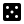
\includegraphics[width=4mm]{out/pdf/svg/dice5.pdf}
after six rolls}}}

\begin{center}
\def\svgwidth{0.4\textwidth}
{\scriptsize\input{out/tex/svg/ws_analyze_1.pdf_tex}}\hspace{1cm}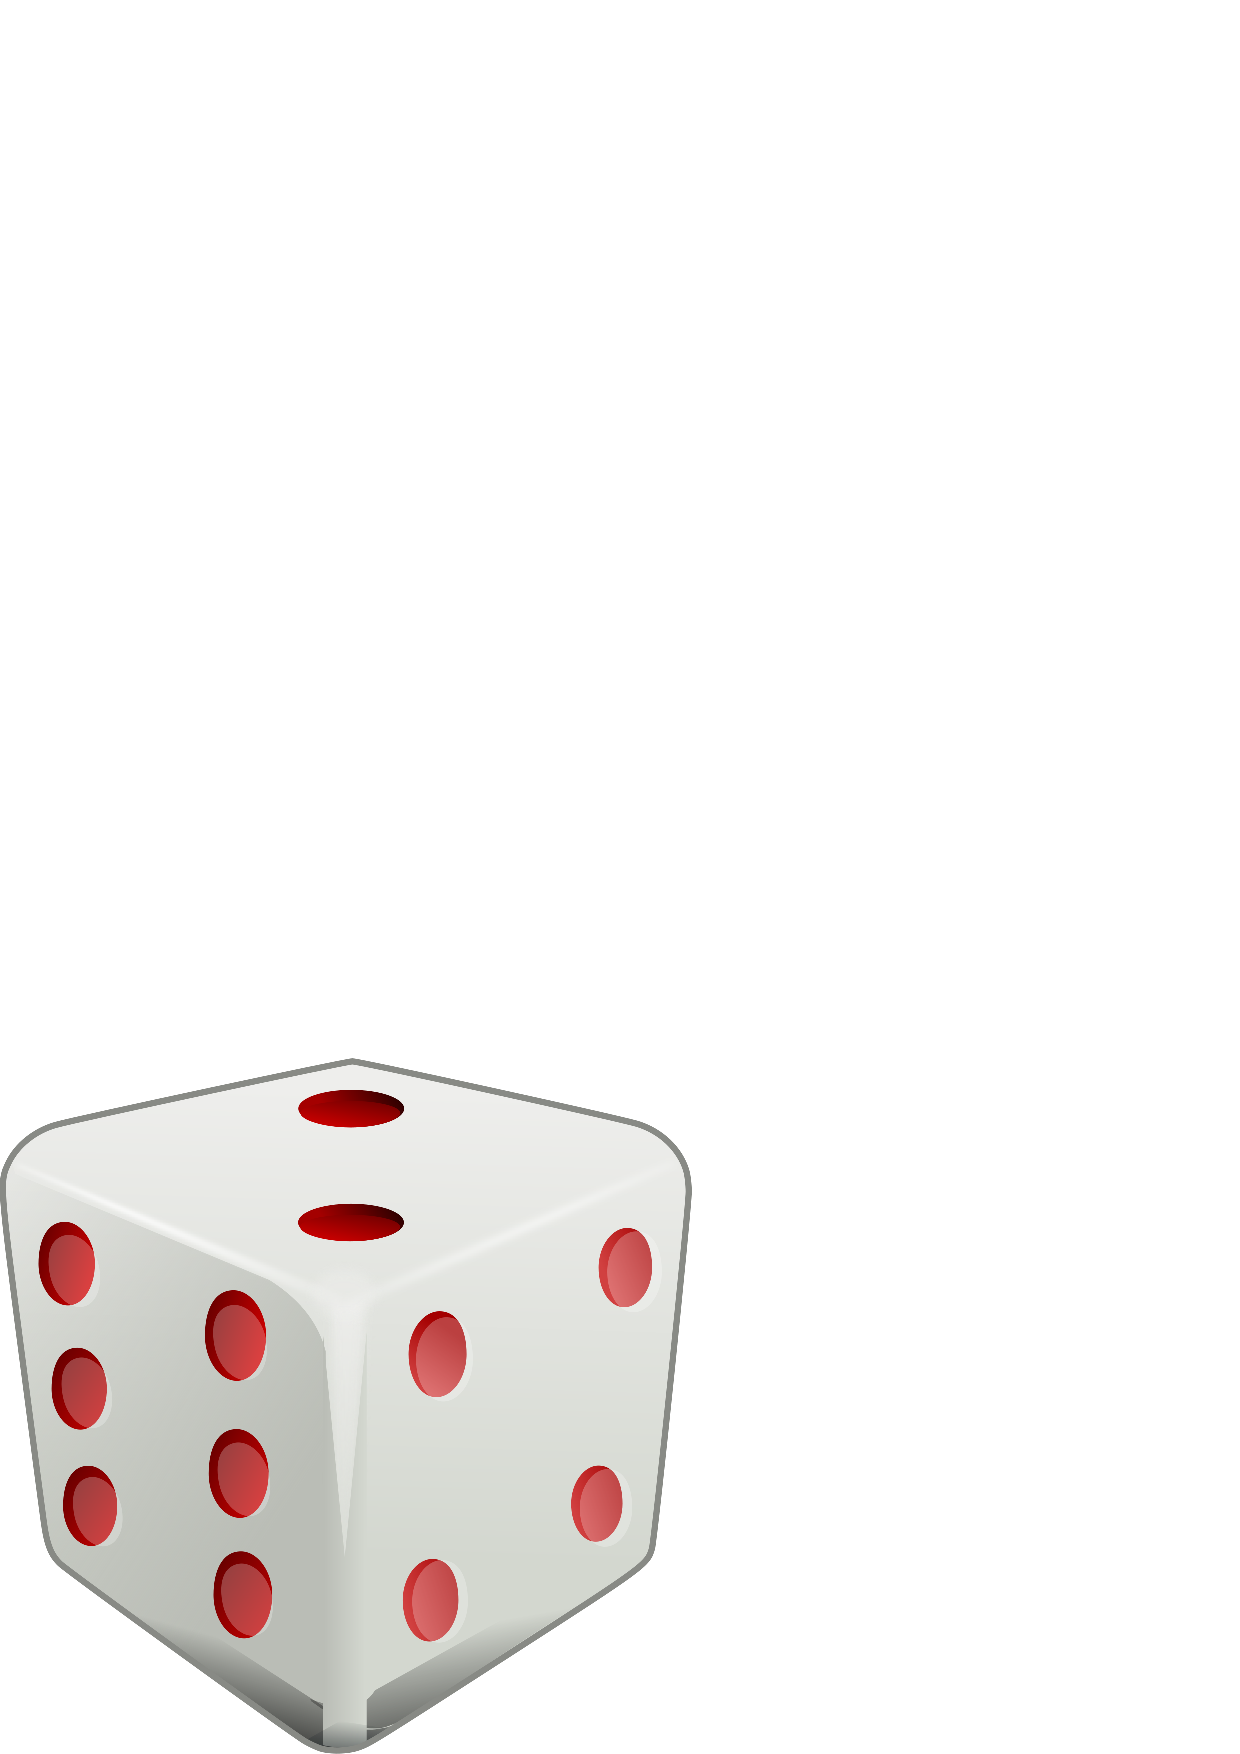
\includegraphics[width=2cm]{out/pdf/svg/dice.pdf}
\end{center}

\item<3-> we are going to extend the argument to {\em
    any} ready task along a ready path, and establish an
  average number of steal attempts for any ready
  task to get executed
\end{itemize}
\end{frame}


%%%%%%%%%%%%%%%%% 
\begin{frame}
\frametitle{How many steal attempts to occur for {\em any} ready task to get executed?}
\begin{columns}
\begin{column}{0.5\textwidth}
\begin{itemize}
\only<1>{
\item there are five types of edges
  \begin{itemize}
  \item [(A)] create\_task $\rightarrow$ child
  \item [(B)] create\_task $\rightarrow$ the continuation
  \item [(C)] wait\_task $\rightarrow$ the continuation
  \item [(D)] last node of a task $\rightarrow$ the parent's continuation after the corresponding wait
  \item [(E)] non-task node $\rightarrow$ the continuation
  \end{itemize}}
\only<2>{
\item the successor of type (A), (C), (D), and (E) is executed
  immediately after the predecessor is executed.

\emph{\ao{there are no delays on edges of these types}}}
\only<3>{
\item only the successor of type (B) edges 
  may need a steal attempt to get executed
\item as has been discussed, once a task is at the bottom
  of a deque, it needs $\approx P$ steal attempts
  on average until it gets stolen
}
\only<4>{
\item note that a successor of a type (B) edge 
  (continuation of a task creation) is not necessarily 
  at the bottom of a deque
\item e.g., $y$ cannot be stolen until $x$ has been stolen
}
\only<5>{
\item stealing such a task requires an accordingly many steal attempts
\item e.g., stealing $y$ requires $2P$ attempts on average 
  ($P$ to steal $x$ and another $P$ to steal $y$)
}
\end{itemize}
\end{column}
\begin{column}{0.5\textwidth}
\begin{center}
\only<1>{\def\svgwidth{\textwidth}{\scriptsize\input{out/tex/svg/ws_analyze_2.pdf_tex}}}%
\only<2>{\def\svgwidth{\textwidth}{\scriptsize\input{out/tex/svg/ws_analyze_3.pdf_tex}}}%
\only<3>{\def\svgwidth{\textwidth}{\scriptsize\input{out/tex/svg/ws_analyze_4.pdf_tex}}}%
\only<4->{\def\svgwidth{\textwidth}{\scriptsize\input{out/tex/svg/ws_analyze_5.pdf_tex}}}%
\end{center}
\end{column}  
\end{columns}
\end{frame}


%%%%%%%%%%%%%%%%% 
\begin{frame}
\frametitle{When a task becomes stealable?}

\begin{columns}
\begin{column}{0.7\textwidth}

\begin{itemize}

\item<1-> in general, in order for the continuation of
  a {\tt create\_task} ($n$) to be stolen, 
  continuations of all {\tt create\_task}s
  along the path from the start node to $n$
  must be stolen

% \item<2-> so we define a node $n$ to be \ao{\em critical} iff
%   \begin{itemize}
%   \item it is ready and
%   \item for all {\tt create\_task} 
%     nodes along the path from the start node to $n$,
%     its continuation node has been executed
%   \end{itemize}

\end{itemize}

\end{column}
\begin{column}{0.3\textwidth}
\def\svgwidth{0.6\textwidth}{\scriptsize\input{out/tex/svg/ws_analyze_critical.pdf_tex}}
\end{column}
\end{columns}

% \begin{itemize}
% \item<3-> then we have a critical node is at the bottom of a deque; and
% \item<3-> a critical node is, 
%   on average, executed within $P$ steal attempts
% \end{itemize}

\end{frame}

%%%%%%%%%%%%%%%%% 
\begin{frame}
\frametitle{Summary of the proof}
Now we have all ingredients to finish the proof

\begin{itemize}
\item<1-> [] the average number of steal attempts to finish the ready path
\item<2-> [] $\approx P \times \mbox{the length of the ready path}$
\item<3-> [] $\leq P T_\infty$
\end{itemize}

therefore, 

\[ \mbox{average of } T_p \leq \frac{T_1 + P T_\infty}{P} = \frac{T_1}{P} + T_\infty \]

\end{frame}

\iffalse
%%%%%%%%%%%%%%%%% 
\begin{frame}
\frametitle{Summary of the proof}
\begin{itemize}
\item<1-> [(1)] there is a ready path
\item<2-> [(2)] define a critical node as in the previous slide
\item<3-> [(3)] with this definition
  a critical node will be stolen, on average, within $P$ steal attempts
\item<4-> [(4)] a critical node will be executed 
  one time step after stolen, 
  so will be finished within $2P$ steal attempts
\item<5-> [(5)] the length of any ready path is $\leq T_\infty$
\item<6-> [(6)] from (4) and (5), any path will take $2 T_\infty P$ steal attempts to finish
\item<7-> [(7)] therefore 
\[ E(T_P) \leq \frac{T_1 + 2T_\infty P}{P} \leq \frac{T_1}{P} + 2T_\infty \]
\end{itemize}
\end{frame}
\fi

%%%%%%%%%%%%%%%%% 
\begin{frame}
\frametitle{Extensions}
\begin{itemize}
\item we assumed a steal attempt takes a single time step, 
  but it can be generalized to a setting where 
  a steal attempt takes $a$ time steps,
\[ E(T_P) \leq \frac{T_1}{P} + aT_\infty \]

\item we can also probabilistically bound the execution time
\item the basis is the probability that a critical node 
  takes $cP$ steal attempts to be executed is $\leq e^{-c}$
\begin{equation*}
\because \left(1 - \frac{1}{P}\right)^{cP} \leq e^{-c}
\end{equation*}

\item based on this we bound the probability that
  a path of length $l$ takes $ClP$ steal
  attempts, for a large enough constant $C$

\end{itemize}

\end{frame}

%=================================

%=================================


%=================================
\section{Analyzing cache misses of work stealing}
%=================================
%%%%%%%%%%%%%%%%% 
\begin{frame}[fragile]
\frametitle{Analyzing cache misses of work stealing}
\begin{itemize}

\item<1-> we like to know the amount of data transfers
  between a processor's cache and \{ main memory,
  other caches \}, under a task parallel scheduler

\item<2-> in particular, we like to understand how much can it be
worse (or better) than its serial execution 

\begin{center}
\includegraphics[width=0.7\textwidth]{out/pdf/svg/ws_cache_goals.pdf}
\end{center}
\end{itemize}
\end{frame}


%%%%%%%%%%%%%%%%% 
\begin{frame}
\frametitle{An analysis methodology of serial computation}
\begin{columns}
\begin{column}{0.6\textwidth}
\begin{itemize}
\item<1-> we have learned how to analyze data transfer
  between the cache and main memory, in single
  processor machines
\item<2-> the key was to identify ``cache-fitting'' subcomputations
  (working set size $\leq$ $C$ words); and
\item<3-> a cache-fitting subcomputation 
  induces $\leq C$ words data transfers
\end{itemize}
\end{column}

\begin{column}{0.4\textwidth}
\def\svgwidth{\textwidth}
{\scriptsize\input{out/tex/svg/cache_model.pdf_tex}}

\vskip1cm

\def\svgwidth{\textwidth}
{\scriptsize\input{out/tex/svg/analyze_cache.pdf_tex}}
\end{column}
\end{columns}
\end{frame}

%%%%%%%%%%%%%%%%% 
\begin{frame}
\frametitle{Minor remarks (data transfer vs. cache misses)}
\begin{itemize}
\item we hereafter use ``a single cache miss'' to mean
  ``a single data transfer from/to a cache''
\item in real machines, some data transfers do not induce
  to cache misses due to prefetches
\item we say ``cache misses'' for simplicity
\end{itemize}

\end{frame}

%%%%%%%%%%%%%%%%% 
\begin{frame}[fragile]
\frametitle{What's different in parallel execution?}
\begin{columns}
\begin{column}{0.7\textwidth}
\begin{itemize}
\item<1-> the argument that ``cache misses by 
  a cache-fitting subcomputation $\leq$ $C$''
  no longer holds in parallel execution
\item<2-> consider two subcomputations $A$ and $B$
\begin{lstlisting}
create_task({ @$A$@ });
@$B$@
\end{lstlisting}
\begin{itemize}
\item assume $A$ and $B$ together fit in the cache
\item even so, if $A$ and $B$
  are executed on different processors, 
  originally a cache hit in $B$ may miss
\end{itemize}
\end{itemize}
\end{column}

\begin{column}{0.3\textwidth}
\def\svgwidth{\textwidth}
{\footnotesize \input{out/tex/svg/explain_extra_cache_miss.pdf_tex}}
\end{column}
\end{columns}
\end{frame}

%%%%%%%%%%%%%%%%% 
\begin{frame}[fragile]
\frametitle{What's different in parallel execution?}

\begin{itemize}
\item so a parallel execution might increase cache
  misses
\item but how much? 

{\footnotesize {\it The data locality of work stealing.}  SPAA
'00 Proceedings of the twelfth annual ACM
symposium on Parallel algorithms and
architectures.}
\end{itemize}
\end{frame}

%%%%%%%%%%%%%%%%% 
\begin{frame}[fragile]
\frametitle{Problem settings}
\begin{itemize}
\item $P$ processors ($\equiv$ $P$ workers)
\item caches are \ao{\em private} to each processor
  (no shared caches)
\item consider only a single-level cache, 
  with the capacity of $C$ words
\item \ao{\em LRU replacement:} i.e., a cache holds most
  recently accessed $C$ distinct words
\end{itemize}

\begin{center}
\def\svgwidth{0.7\textwidth}
{\scriptsize\input{out/tex/svg/ws_cache_model.pdf_tex}}
\end{center}
\end{frame}

%%%%%%%%%%%%%%%%% 
\begin{frame}
\frametitle{The key observation}
\begin{columns}
\begin{column}{0.7\textwidth}
\begin{itemize}
\item we have learned the work stealing scheduler 
  tends to preserve much of the serial execution order 

\item $\Rightarrow$ extra cache misses are caused
  by work stealings

\item a work stealing essentially brings a
  subcomputation to \aka{\em a processor with
    unknown cache states}
\end{itemize}
\end{column}

\begin{column}{0.3\textwidth}
\def\svgwidth{\textwidth}
{\footnotesize \input{out/tex/svg/ws_cache_analysis_observation.pdf_tex}}
\end{column}
\end{columns}
\end{frame}


%%%%%%%%%%%%%%%%% 
\begin{frame}
\frametitle{The key questions}
\begin{itemize}
\item \ao{key question 1:} how many \ao{\em extra}
  misses can occur when a subcomputation moves to
  an unknown cache states?

\begin{center}
\def\svgwidth{0.7\textwidth}
{\scriptsize\input{out/tex/svg/ws_cache_miss_analysis_clues.pdf_tex}}
\end{center}

\item \ao{key question 2:} how many times work
  stealings happen? (we know an answer)
\end{itemize}
\end{frame}

%%%%%%%%%%%%%%%%% 
\begin{frame}
\frametitle{Roadmap}

\begin{itemize}
\item [(1)] bound the number of extra cache misses that occurs
  each time a node is \ao{\em drifted} 
  (i.e., executed in a different order with the serial execution)

\item [(2)] we know an upper bound on the number of steals
\item [(3)] from (2), bound the number of drifted nodes
\item combine (1) and (3) to derive an upper bound on 
  the total number of extra cache misses
\end{itemize}
\end{frame}

%%%%%%%%%%%%%%%%% 
\begin{frame}
\frametitle{Extra misses per drifted node}
\begin{itemize}
\item when caches are LRU, the two cache states
  converge to an identical state, after no more
  than $C$ cache misses occur in either cache

\begin{center}
\def\svgwidth{0.7\textwidth}
{\scriptsize\input{out/tex/svg/ws_cache_miss_analysis_clues_ans.pdf_tex}}
\end{center}

\item this is because the cache is LRU (holds
  most recently accessed distinct $C$ words)

\[ 
\therefore \mbox{\ao{\em extra cache misses for each drifted node}} \leq C 
\]
\end{itemize}
\end{frame}

%%%%%%%%%%%%%%%%% 
\begin{frame}
\frametitle{A bound on the drifted nodes}

\begin{columns}
\begin{column}{0.55\textwidth}
\begin{itemize}
\item let $v$ a node in the DAG and $u$ the node
  that would immediately precedes $v$ in the
  serial execution

\item we say $v$ is \ao{\em drifted} when $u$ and
  $v$ are not executed consecutively on the same
  processor
\end{itemize}
\end{column}

\begin{column}{0.45\textwidth}
\begin{center}
\def\svgwidth{0.9\textwidth}
{\scriptsize\input{out/tex/svg/chol_dag_drifted.pdf_tex}}
\end{center}
\end{column}
\end{columns}

\begin{itemize}
\item without a detailed proof, we note:
\[
  \begin{array}{ll}
& \mbox{\em the number of drifted nodes in the work stealing scheduler} \\
\leq & 2 \times \mbox{\em the number of steals} 
  \end{array}
\]
\end{itemize}
\end{frame}

%%%%%%%%%%%%%%%%% 
\begin{frame}
\frametitle{The main result}
\begin{itemize}
\item the average number of work stealings $\approx PT_\infty$ 
\item $\Rightarrow$ the average number of drifted nodes
  $\approx 2PT_\infty$ 
\item $\Rightarrow$ the average number of extra cache misses
  $\leq 2CPT_\infty$ 
\item average execution time
\[ T_P \leq \frac{T_1}{P} + 2m CT_\infty, \]
where $m$ is the cost of a single cache miss
\end{itemize}
\end{frame}

%=================================
\section{Summary}
%=================================
%%%%%%%%%%%%%%%%% 
\begin{frame}
\frametitle{Summary}

\begin{itemize}
\item the basics of work stealing scheduler
  \begin{itemize}
  \item work-first (preserve serial execution order)
  \item steal tasks from near the root
  \end{itemize}
\item average execution time (without cost of communication)
\[ T_P \leq \frac{T_1}{P} + T_\infty \]
\item with the cost of communication
\[ T_P \leq \frac{T_1}{P} + 2mCT_\infty \]
where $mC$ essentially represents the time to fill the cache
\end{itemize}
\end{frame}

\end{document}
